\acrodef{CGL}{Cut Generation Library}
\begin{sloppypar} By default \ac{DIP} uses the \ac{CGL} to add cuts. We can use \lstinline{dippyOpts} to turn off \ac{CGL} cuts and observe how effective the \ac{CGL} are
\lstinputlisting[firstnumber=73,linerange={107-108,110-110,115-117}]{../../examples/Dippy/bpp/bin_pack_func.py}
The branch-and-bound tree is significantly larger (see figure \ref{fig:bpp_tree4}) than the original branch-and-bound tree that only used \ac{CGL} cuts (see figure \ref{fig:bpp_tree1}).
\begin{figure}[htp]
\begin{center}
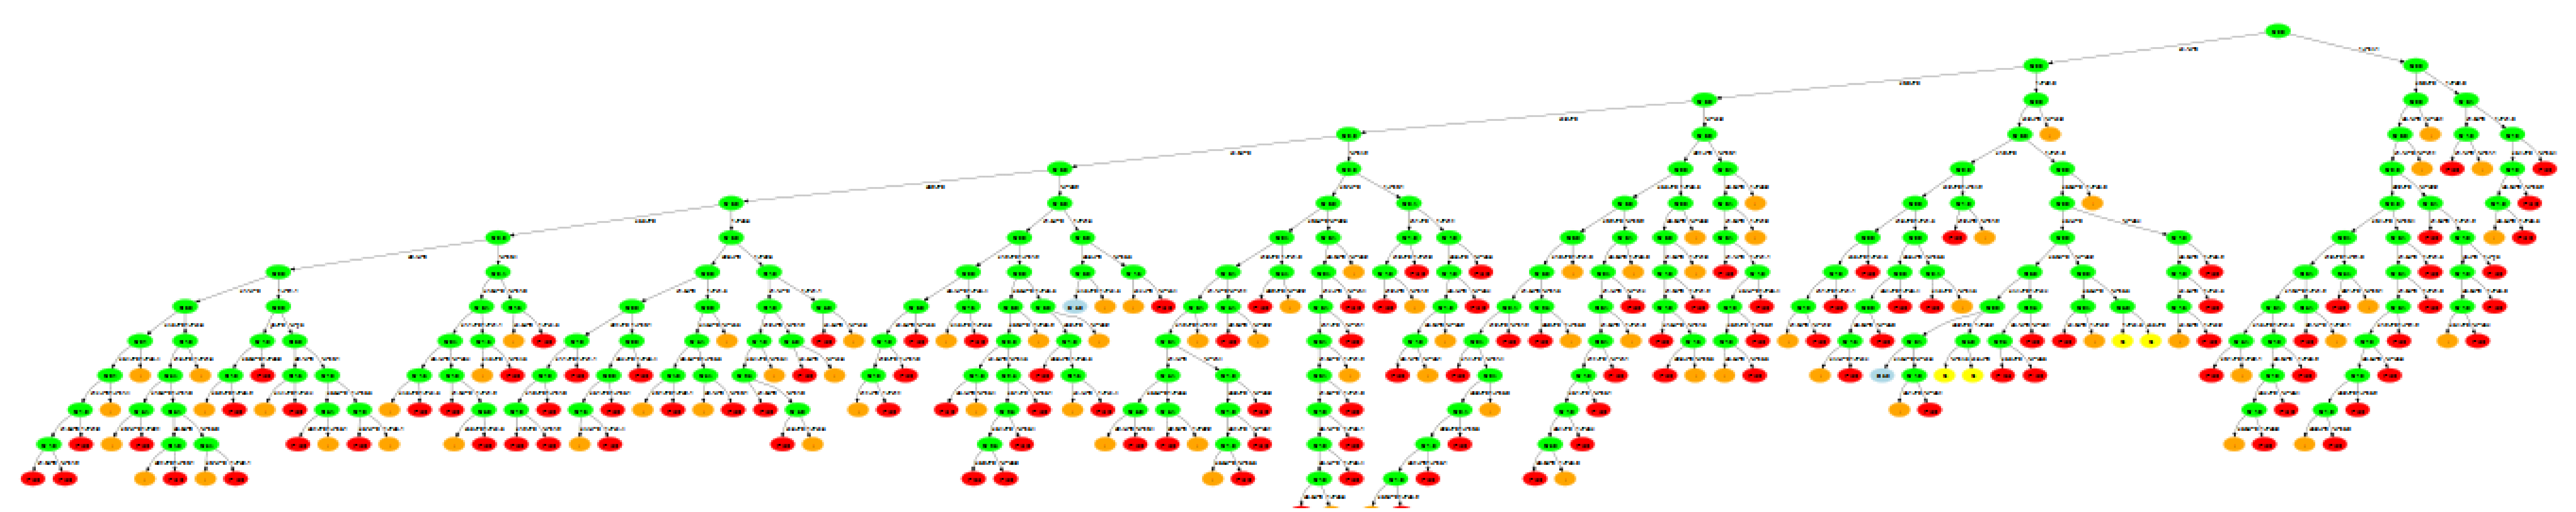
\includegraphics[scale=0.075]{img/bpp_tree4.eps}
\end{center}
\caption{Branch-and-bound tree for bin packing problem instance without \ac{CGL} cuts.} \label{fig:bpp_tree4}
\end{figure}


To add user-defined cuts in Dippy, we first define a new procedure for generating cuts and (if necessary) a procedure for determining a feasible solution.
Within Dippy, this requires two new functions, \lstinline{generate_cuts} and \lstinline{is_solution_feasible}.
As in \sbsref{sbs:branch}, the embedded bin packing problem and decisions variables make it easy to access the solution values of variables in the bin packing problem.
The inputs to \lstinline{is_solution_feasible} are:
\begin{enumerate}
\item \lstinline{prob} -- the \lstinline{DipProblem} being solved;
\item \lstinline{sol} -- an indexable object representing the solution at the current node;
\item \lstinline{tol} -- the zero tolerance value.
\end{enumerate}
and the inputs to \lstinline{generate_cuts} are:
\begin{enumerate}
\item \lstinline{prob} -- the \lstinline{DipProblem} being solved;
\item \lstinline{node} -- various properties of the current node, including the solution.
\end{enumerate}

If a solution is determined to be infeasible either by \ac{DIP} (for example some integer variables are fractional) or by \lstinline{is_solution_feasible} (which is useful for solving problems like the travelling salesman problem with cutting plane methods), cuts will be generated by \lstinline{generate_cuts} and the in-built \ac{CGL} (if enabled).\end{sloppypar}

\begin{comment}

Marchand and Wolsey \cite{agg_mir2001} define many types of cuts for \ac{MILP} problems.
One of these is the \textit{weighted inequality}.
For each facility location $i$ and some subset $S_i (\subseteq \{1, \ldots, n \})$ of the products we can calculate
\[ \mu_i = C - \sum_{j \in S_i} w_j x_{ij} \]
and use it to generate a weighted inequality
\[ \sum_{j \in S_i} w_j x_{ij} + \sum_{j \notin S_i} (w_j - \mu_i)^+ x_{ij} \leq C - \mu _i \]
which forms a valid inequality for the facility location problem.

The cut generating function creates the subsets $S_i$ for each location from the fractional solution in a greedy way depending on the $x_{ij}$ values, and from these we generate a set of weighted inequality cuts.
The code listing below shows how to build the set of cuts, and omits the generation of $S_i$ for the sake of brevity.
\lstinputlisting[firstnumber=67,linerange=67-74]{../../examples/Dippy/bpp/bin_pack_func.py}
$\vdots$\newpage
\lstinputlisting[firstnumber=98,linerange=98-111]{../../examples/Dippy/bpp/bin_pack_func.py}

Adding the weighted inequality cut generator reduces the branch-and-bound tree size from 419 nodes to 77 nodes.

\end{comment}